\documentclass[
	%a4paper, % Use A4 paper size
	letterpaper, % Use US letter paper size
]{jdf}

\addbibresource{references.bib}

\author{Qiyun Zhao}
\email{qzhao97@gatech.edu}
\title{AI, Ethics, Society\\Homework Project \#2}

\begin{document}
%\lsstyle
\maketitle

\section{Explore the data}
\subsection{Selected Dataset}
hospital-discharge-2017.csv \newline
New York Hospital Inpatient Discharge Information in 2017: https://health.data.ny.gov/dataset/Hospital-Inpatient-Discharges-SPARCS-De-Identified/22g3- z7e7
\subsection{Number of observations: 1048575}
\subsection{Number of variables in the dataset: 18}
\subsection{Regulated Domain in Law: Yes}
Hospital is a public accommodation. (Civil Rights Act of 1964)
\subsection{Number of Protected Class Variables}
There are four protected class variables.
\begin{jdftable}
\captionof{table}{variables associated with a protected class}\label{table:Example}
\small % Reduce font size
\begin{tabular}{@{} L{0.15\linewidth} c L{0.52\linewidth}}
\textbf{Name} & \textbf{Protected Class} & \textbf{LAW} \\
	\toprule[0.5pt]
	Age Group & Age & Age Discrimination in Employment Act of 1967\\
	\midrule
	Gender & Sex & Equal Pay Act of 1963; Civil Rights Act of 1964, 1991 \\
	\midrule
	Race &Race & Civil Rights Act of 1964, 1991\\
	\midrule
	Ethnicity & National origin &Civil Rights Act of 1964, 1991\\
\end{tabular}
\end{jdftable}

\break
\section{relationships between dependent and independent variables}
\subsection{Output for Length of Stay-Age Group Combination}
\ 
\begin{jdftable}
\captionof{table}{Frequesncy of Length of Stay associated with Age}\label{table:Example}
\small % Reduce font size
\begin{tabular}{@{} l c c c c c c}
\textbf{Independent Variable} & \textbf{Dependent Variable-Length of Stay} &\textbf{days} & & & \\
	\toprule[0.5pt]
	Age Group & (0, 2] & (2, 5] & (5, 10] & (10, 20] & (20, 50] & (50, 120] \\
\midrule
0 to 17 & 89723 & 45734 & 9093 & 4672 & 2809 & 1159 \\
\midrule
18 to 29 & 45997 & 39526 & 10217 & 5353 & 2518 & 440 \\
\midrule
30 to 49 & 83813 & 75010 & 23069 & 11628 & 5365 & 895 \\
\midrule
50 to 69 & 103674 & 98963 & 52460 & 26431 & 11054 & 1895 \\
\midrule
70 or Older & 75863 & 109588 & 69977 & 31019 & 9478 & 1152 \\
\end{tabular}
\end{jdftable}
\begin{jdffigure}
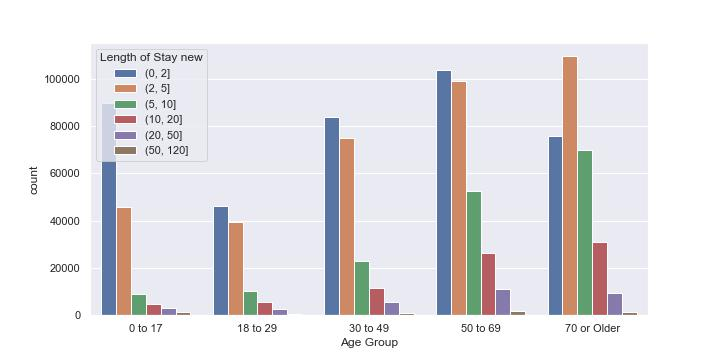
\includegraphics[height=13cm]{Figures/length-age.jpg} \\
\captionof{figure}{Length of Stage associated with Age}\label{fig:length-age}%
\end{jdffigure}

\subsection{Output for Length of Stay-Gender Combination}
\ 
\begin{jdftable}
\captionof{table}{Frequesncy of Length of Stay associated with Gender}\label{table:Example}
\small % Reduce font size
\begin{tabular}{@{} l c c c c c c}
\textbf{Independent Variable} & \textbf{Dependent Variable-Length of Stay} &\textbf{days} & & & \\
	\toprule[0.5pt]
Gender & (0, 2] & (2, 5] & (5, 10] & (10, 20] & (20, 50] & (50, 120] \\ \midrule
F & 224687 & 216534 & 85795 & 38214 & 14196 & 2400 \\ \midrule
M & 174371 & 152283 & 79018 & 40889 & 17028 & 3140 \\ \midrule
U & 12 & 4 & 3 & 0 & 0 & 1 \\
\end{tabular}
\end{jdftable}
\begin{jdffigure}
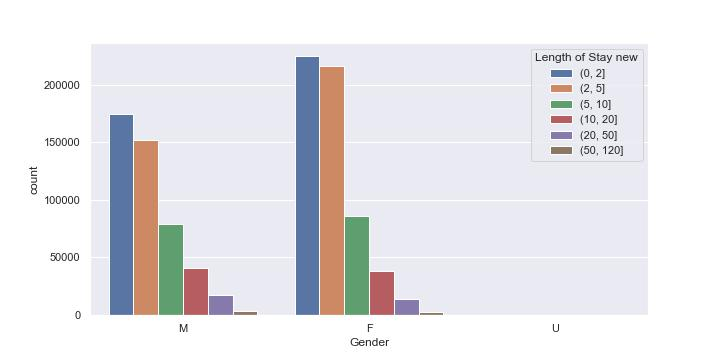
\includegraphics[height=13cm]{Figures/length-gender.jpg} \\
\captionof{figure}{Length of Stage associated with Gender}\label{fig:length-gender}%
\end{jdffigure}
\subsection{Output for Length of Stay-Race Combination}
\ 
\begin{jdftable}
\captionof{table}{Frequesncy of Length of Stay associated with Race}\label{table:Example}
\small % Reduce font size
\begin{tabular}{@{} l c c c c c c}
\textbf{Independent Variable} & \textbf{Dependent Variable-Length of Stay} &\textbf{days} & & & \\
	\toprule[0.5pt]
Race & (0, 2] & (2, 5] & (5, 10] & (10, 20] & (20, 50] & (50, 120] \\ 
\midrule
Black/African American & 67009 & 66274 & 31901 & 17515 & 7451 & 1478 \\
\midrule
Multi-racial & 3917 & 3644 & 1551 & 711 & 295 & 73 \\
\midrule
Other Race & 110102 & 92612 & 35346 & 17708 & 7567 & 1692 \\
\midrule
White & 218042 & 206291 & 96018 & 43169 & 15911 & 2298 \\
\end{tabular}
\end{jdftable}
\begin{jdffigure}
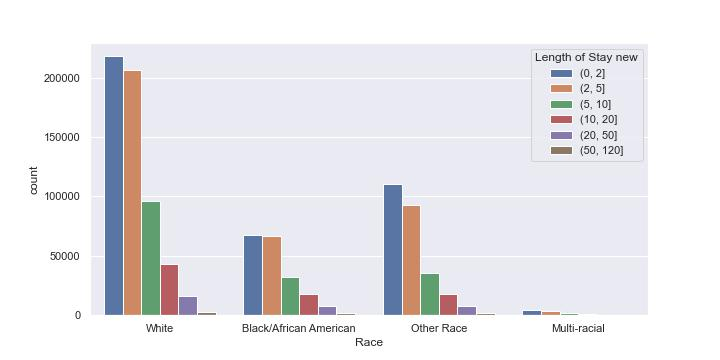
\includegraphics[height=13cm]{Figures/length-race.jpg} \\
\captionof{figure}{Length of Stage associated with Race}\label{fig:length-race}%
\end{jdffigure}
\subsection{Output for Length of Stay-Ethnicity Combination}
\ 
\begin{jdftable}
\captionof{table}{Frequesncy of Length of Stay associated with Ethnicity}\label{table:Example}
\small % Reduce font size
\begin{tabular}{@{} l c c c c c c}
\textbf{Independent Variable} & \textbf{Dependent Variable-Length of Stay} &\textbf{days} & & & \\
	\toprule[0.5pt]
Ethnicity & (0, 2] & (2, 5] & (5, 10] & (10, 20] & (20, 50] & (50, 120] \\
\midrule
Multi-ethnic & 1606 & 1398 & 485 & 242 & 104 & 30 \\
\midrule
Not Span/Hispanic & 316125 & 297774 & 138096 & 65691 & 25612 & 4357 \\
\midrule
Spanish/Hispanic & 54884 & 47488 & 17154 & 8220 & 3303 & 655 \\
\midrule
Unknown & 26455 & 22161 & 9081 & 4950 & 2205 & 499 \\
\end{tabular}
\end{jdftable}
\begin{jdffigure}
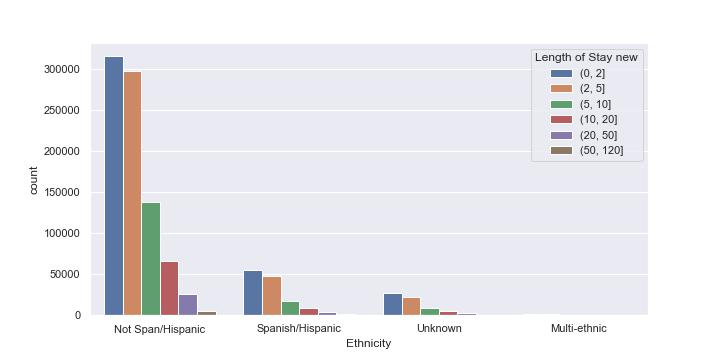
\includegraphics[height=13cm]{Figures/length-Ethnicity.jpg} \\
\captionof{figure}{Length of Stage associated with Ethnicity}\label{fig:length-Ethnicity}%
\end{jdffigure}
\subsection{Output for APR Severity of Illness Code-Age Group Combination}
\ 
\begin{jdftable}
\captionof{table}{Frequesncy of APR Severity of Illness Code associated with Age}\label{table:Example}
\small % Reduce font size
\begin{tabular}{@{} l c c c c c}
\textbf{Independent Variable} & \textbf{Dependent Variable-Illness Code} & & & & \\
	\toprule[0.5pt]
	Age Group & 0 & 1 & 2 & 3 & 4\\
	\midrule
	0 to 17 & 78 & 99272 & 36546 & 14307 & 2987 \\
 \midrule
 18 to 29 & 5 & 49274 & 42544 & 10391 & 1837 \\
 \midrule
 30 to 49 & 5 & 81573 & 84202 & 28537 & 5463 \\
 \midrule
 50 to 69 & 0 & 71624 & 124930 & 78954 & 18969 \\
 \midrule
 70 or Older & 0 & 40790 & 117901 & 109562 & 28824 \\
\end{tabular}
\end{jdftable}

\begin{jdffigure}
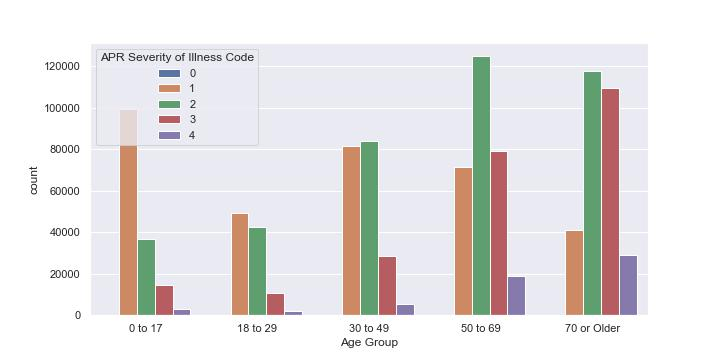
\includegraphics[height=13cm]{Figures/code-age.jpg} \\
\captionof{figure}{APR Severity of Illness Code associated with Age}\label{fig:code-age}%
\end{jdffigure}
\subsection{Output for APR Severity of Illness Code-Gender Combination}
\ 
\begin{jdftable}
\captionof{table}{Frequesncy of APR Severity of Illness Code associated with Gender}\label{table:Example}
\small % Reduce font size
\begin{tabular}{@{} l c c c c c}
\textbf{Independent Variable} & \textbf{Dependent Variable-Illness Code} & & & & \\
	\toprule[0.5pt]
	Gender & 0 & 1 & 2 & 3 & 4 \\
\midrule
F & 47 & 204335 & 225867 & 124164 & 27413 \\
\midrule
M & 41 & 138187 & 180251 & 117584 & 30666 \\
\midrule
U & 0 & 11 & 5 & 3 & 1 \\
\end{tabular}
\end{jdftable}

\begin{jdffigure}
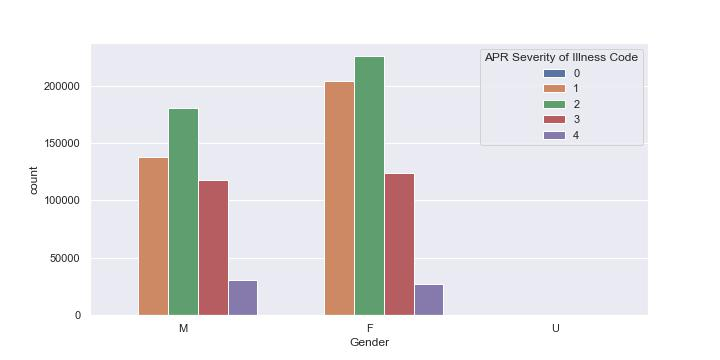
\includegraphics[height=13cm]{Figures/code-gender.jpg} \\
\captionof{figure}{APR Severity of Illness Code associated with Gender}\label{fig:code-gender}%
\end{jdffigure}

\subsection{Output for APR Severity of Illness Code-Race Combination}
\ 
\begin{jdftable}
\captionof{table}{Frequesncy of APR Severity of Illness Code associated with Race}\label{table:Example}
\small % Reduce font size
\begin{tabular}{@{} l c c c c c}
\textbf{Independent Variable} & \textbf{Dependent Variable-Illness Code} & & & & \\
	\toprule[0.5pt]
Race & 0 & 1 & 2 & 3 & 4 \\
\midrule
Black/African American & 25 & 54922 & 80158 & 46360 & 10163 \\
\midrule
Multi-racial & 3 & 3119 & 3757 & 2646 & 666 \\
\midrule
Other Race & 39 & 101980 & 97947 & 52135 & 12926 \\
\midrule
White & 21 & 182512 & 224261 & 140610 & 34325 \\
\end{tabular}
\end{jdftable}

\begin{jdffigure}
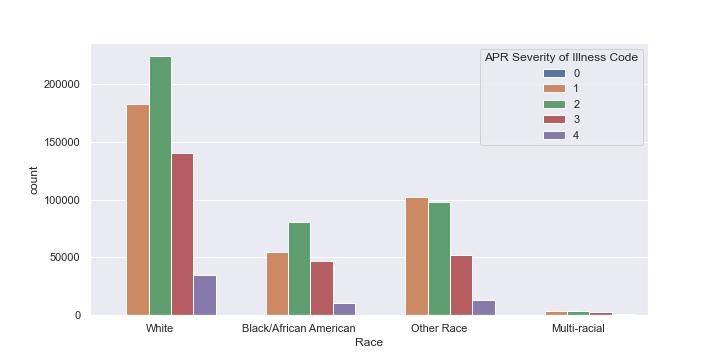
\includegraphics[height=13cm]{Figures/code-race.jpg} \\
\captionof{figure}{APR Severity of Illness Code associated with Race}\label{fig:code-race}%
\end{jdffigure}

\subsection{Output for APR Severity of Illness Code-Ethnicity Combination}
\ 
\begin{jdftable}
\captionof{table}{Frequesncy of APR Severity of Illness Code associated with Ethnicity}\label{table:Example}
\small % Reduce font size
\begin{tabular}{@{} l c c c c c}
\textbf{Independent Variable} & \textbf{Dependent Variable-Illness Code} & & & & \\
	\toprule[0.5pt]
Ethnicity & 0 & 1 & 2 & 3 & 4 \\
\midrule
Multi-ethnic & 0 & 1397 & 1324 & 938 & 206 \\
\midrule
Not Span/Hispanic & 54 & 266442 & 329128 & 202722 & 49309 \\
\midrule
Spanish/Hispanic & 18 & 49345 & 52072 & 25163 & 5106 \\
\midrule
Unknown & 16 & 25349 & 23599 & 12928 & 3459 \\
\end{tabular}
\end{jdftable}

\begin{jdffigure}
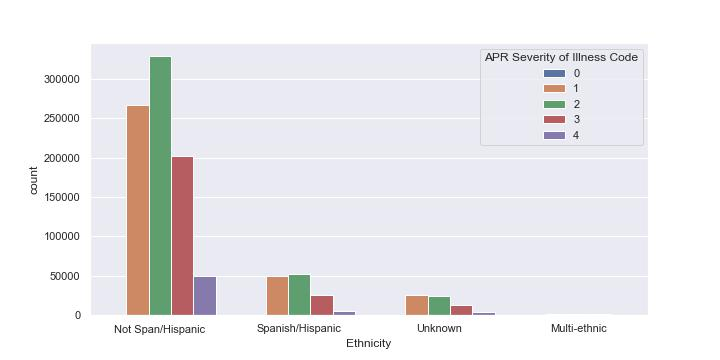
\includegraphics[height=13cm]{Figures/code-Ethnicity.jpg} \\
\captionof{figure}{APR Severity of Illness Code associated with Ethnicity}\label{fig:code-Ethnicity}%
\end{jdffigure}



\section{Manipulate with data}

\subsection{Fair Hypothesis}
As seen from this graph, APR Severity of Illness Code is not dependent on the Age Group. [Manipulations: Scale the y-axis to $10^7$].
\begin{jdffigure}
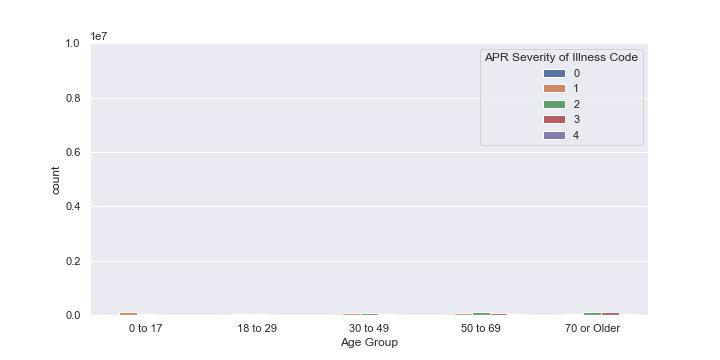
\includegraphics[height=13cm]{Figures/code-age-fair.jpg} \\
\captionof{figure}{Fair Hypothesis for APR Severity of Illness Code with Age Group}\label{fig:code-age-fair}%
\end{jdffigure}
\subsection{Bias Hypothesis}
As seen from this graph,  APR Severity of Illness Codes are significantly dependent on the Age Group. [This hypothesis was easily supported with the data so didn’t require much in manipulations: Used bar graph; Reduced Scale; Reworded labels].
\begin{jdffigure}
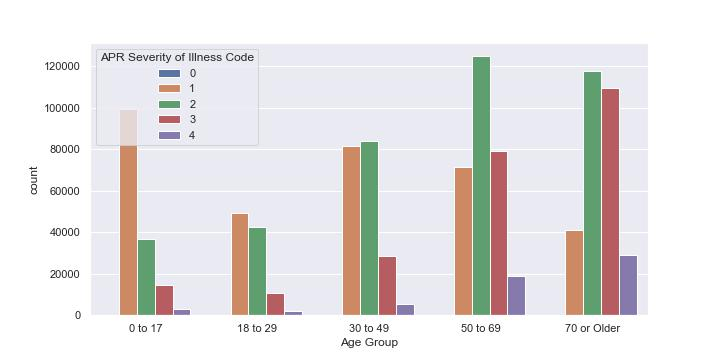
\includegraphics[height=13cm]{Figures/code-age.jpg} \\
\captionof{figure}{Bias Hypothesis for APR Severity of Illness Code with Age Group}\label{fig:code-age-fair}%
\end{jdffigure}

\section{Comparison of the original dataset and reduced dataset}
\subsection{Comparison for Length of Stay and Age Group}
There are small difference in Mean between original data and reduced data. But no difference between median and mode. 

\begin{jdftable}
\captionof{table}{APR Severity of Illness Code and Age Group}\label{table:Example}
\small % Reduce font size
\begin{tabular}{@{} l c c c c c}
\textbf{Age Group} & \textbf{0 to 17} &\textbf{18 to 29} & \textbf{30 to 49} & \textbf{50 to 69} & \textbf{70 or older}\\
	\toprule[0.5pt]
APR Severity of Illness Code Mean           &  1.483341 &  1.661522 &  1.789168 &  2.153723 &     2.425546 \\
\midrule
APR Severity of Illness Code Reduced Mean   &  1.483046 &  1.661436 &  1.788435 &  2.153978 &     2.425899 \\
\midrule
Mean Difference                             &  0.000295 &  0.000086 &  0.000733 & -0.000255 &    -0.000353 \\
\midrule
APR Severity of Illness Code Median         &  1.000000 &  2.000000 &  2.000000 &  2.000000 &     2.000000 \\
\midrule
APR Severity of Illness Code Reduced Median &  1.000000 &  2.000000 &  2.000000 &  2.000000 &     2.000000 \\
\midrule
Median Difference                           &  0.000000 &  0.000000 &  0.000000 &  0.000000 &     0.000000 \\
\midrule
APR Severity of Illness Code Mode           &  1.000000 &  1.000000 &  2.000000 &  2.000000 &     2.000000 \\
\midrule
APR Severity of Illness Code Reduced Mode   &  1.000000 &  1.000000 &  2.000000 &  2.000000 &     2.000000 \\
\midrule
Mode Difference                             &  0.000000 &  0.000000 &  0.000000 &  0.000000 &     0.000000 \\
\end{tabular}
\end{jdftable}


\subsection{APR Severity of Illness Code and Age Group}
There are small difference in Mean between original data and reduced data. But no difference between median and mode. 
\begin{jdftable}
\captionof{table}{APR Severity of Illness Code and Gender}\label{table:Example}
\small % Reduce font size
\begin{tabular}{@{} llll}
\textbf{Gender} & \textbf{F} &\textbf{M} & \textbf{U}\\
	\toprule[0.5pt]

APR Severity of Illness Code Mean           &  1.956277 &  2.087089 &  1.700000 \\\midrule
APR Severity of Illness Code Reduced Mean   &  1.955716 &  2.087114 &  1.333333 \\\midrule
Mean Difference                             &  0.000561 & -0.000025 &  0.366667 \\\midrule
APR Severity of Illness Code Median         &  2.000000 &  2.000000 &  1.000000 \\\midrule
APR Severity of Illness Code Reduced Median &  2.000000 &  2.000000 &  1.000000 \\\midrule
Median Difference                           &  0.000000 &  0.000000 &  0.000000 \\\midrule
APR Severity of Illness Code Mode           &  2.000000 &  2.000000 &  1.000000 \\\midrule
APR Severity of Illness Code Reduced Mode   &  2.000000 &  2.000000 &  1.000000 \\\midrule
Mode Difference                             &  0.000000 &  0.000000 &  0.000000 \\
\end{tabular}
\end{jdftable}
\subsection{Length of Stay and Gender}
There are small difference in Mean between original data and reduced data. But no difference between median. Mode is only has small difference in U.  
\begin{jdftable}
\captionof{table}{Length of stay and Gender}\label{table:Example}
\small % Reduce font size
\begin{tabular}{@{} llll}
\textbf{Gender} & \textbf{F} &\textbf{M} & \textbf{U}\\
	\toprule[0.5pt]

Mean           &  5.047232 &  5.917153 &       6.65 \\
\midrule
Reduced Mean   &  5.027059 &  5.937571 &  10.666667 \\
\midrule
Mean Difference                   &  0.020173 & -0.020418 &  -4.016667 \\
\midrule
Median         &       3.0 &       3.0 &        2.0 \\
\midrule
Reduced Median &       3.0 &       3.0 &        2.0 \\
\midrule
Median Difference                 &       0.0 &       0.0 &        0.0 \\
\midrule
Mode           &         2 &         2 &     [1, 2] \\
\midrule
Reduced Mode   &         2 &         2 &          1 \\
\midrule
Mode Difference                   &         0 &         0 &     [0, 1] \\
\end{tabular}
\end{jdftable}



\subsection{APR Severity of Illness Code and Gender}
There are small difference in Mean between original data and reduced data. But no difference between median and mode.  
\begin{jdftable}
\captionof{table}{APR Severity of Illness Code and Gender}\label{table:Example}
\small % Reduce font size
\begin{tabular}{@{} llll}
\textbf{Gender} & \textbf{F} &\textbf{M} & \textbf{U}\\
	\toprule[0.5pt]

APR Severity of Illness Code Mean           &  1.956277 &  2.087089 &  1.700000 \\\midrule
APR Severity of Illness Code Reduced Mean   &  1.955716 &  2.087114 &  1.333333 \\\midrule
Mean Difference                             &  0.000561 & -0.000025 &  0.366667 \\\midrule
APR Severity of Illness Code Median         &  2.000000 &  2.000000 &  1.000000 \\\midrule
APR Severity of Illness Code Reduced Median &  2.000000 &  2.000000 &  1.000000 \\\midrule
Median Difference                           &  0.000000 &  0.000000 &  0.000000 \\\midrule
APR Severity of Illness Code Mode           &  2.000000 &  2.000000 &  1.000000 \\\midrule
APR Severity of Illness Code Reduced Mode   &  2.000000 &  2.000000 &  1.000000 \\\midrule
Mode Difference                             &  0.000000 &  0.000000 &  0.000000 \\
\end{tabular}
\end{jdftable}









\subsection{Length of Stay and Race}
There are small difference in Mean between original data and reduced data. But no difference between median. Mode is only has small difference in U.  
\begin{jdftable}
\captionof{table}{Length of stay and Race}\label{table:Example}
\small % Reduce font size
\begin{tabular}{@{} lrrrr}
\textbf{Race} & \textbf{Black/African American} &\textbf{Multi-racial} & \textbf{Other Race} &\textbf{White}\\
	\toprule[0.5pt]
Length of Stay int Mean           &                6.141728 &      5.476597 &    5.236055 &  5.291151 \\\midrule
Length of Stay int Reduced Mean   &                6.160951 &      5.492871 &    5.229004 &  5.283484 \\\midrule
Mean Difference                   &               -0.019223 &     -0.016274 &    0.007051 &  0.007667 \\\midrule
Length of Stay int Median         &                3.000000 &      3.000000 &    3.000000 &  3.000000 \\\midrule
Length of Stay int Reduced Median &                3.000000 &      3.000000 &    3.000000 &  3.000000 \\\midrule
Median Difference                 &                0.000000 &      0.000000 &    0.000000 &  0.000000 \\\midrule
Length of Stay int Mode           &                2.000000 &      2.000000 &    2.000000 &  2.000000 \\\midrule
Length of Stay int Reduced Mode   &                2.000000 &      2.000000 &    2.000000 &  2.000000 \\\midrule
Mode Difference                   &                0.000000 &      0.000000 &    0.000000 &  0.000000 \\
\end{tabular}
\end{jdftable}










\subsection{APR Severity of Illness Code and Race}
There are small difference in Mean between original data and reduced data. But no difference between median and mode.  
\begin{jdftable}
\captionof{table}{Length of stay and Race}\label{table:Example}
\small % Reduce font size
\begin{tabular}{@{} lrrrr}
\textbf{Race} & \textbf{Black/African American} &\textbf{Multi-racial} & \textbf{Other Race} &\textbf{White}\\
	\toprule[0.5pt]
APR Severity of Illness Code Mean           &                2.061129 &      2.083701 &    1.909175 &  2.045908 \\\midrule
APR Severity of Illness Code Reduced Mean   &                2.062400 &      2.085149 &    1.906669 &  2.046156 \\\midrule
Mean Difference                             &               -0.001271 &     -0.001447 &    0.002506 & -0.000248 \\\midrule
APR Severity of Illness Code Median         &                2.000000 &      2.000000 &    2.000000 &  2.000000 \\\midrule
APR Severity of Illness Code Reduced Median &                2.000000 &      2.000000 &    2.000000 &  2.000000 \\\midrule
Median Difference                           &                0.000000 &      0.000000 &    0.000000 &  0.000000 \\\midrule
APR Severity of Illness Code Mode           &                2.000000 &      2.000000 &    1.000000 &  2.000000 \\\midrule
APR Severity of Illness Code Reduced Mode   &                2.000000 &      2.000000 &    1.000000 &  2.000000 \\\midrule
Mode Difference                             &                0.000000 &      0.000000 &    0.000000 &  0.000000 \\
\end{tabular}
\end{jdftable}
























\subsection{Length of Stay and Ethnicity}
There are small difference in Mean between original data and reduced data. But no difference between median and mode.  
\begin{jdftable}
\captionof{table}{Length of stay and Ethnicity}\label{table:Example}
\small % Reduce font size
\begin{tabular}{@{} lrrrr}
\textbf{Ethnicity} & \textbf{Multi-ethnic} &\textbf{Not Span/Hispanic} & \textbf{Spanish/Hispanic} &\textbf{Unknown}\\
	\toprule[0.5pt]
Length of Stay int Mean           &      5.257697 &           5.495060 &          4.953935 &  5.627488 \\ \midrule
Length of Stay int Reduced Mean   &      5.557858 &           5.497888 &          4.924129 &  5.594485 \\\midrule
Mean Difference                   &     -0.300160 &          -0.002828 &          0.029806 &  0.033004 \\\midrule
Length of Stay int Median         &      3.000000 &           3.000000 &          3.000000 &  3.000000 \\\midrule
Length of Stay int Reduced Median &      3.000000 &           3.000000 &          3.000000 &  3.000000 \\\midrule
Median Difference                 &      0.000000 &           0.000000 &          0.000000 &  0.000000 \\\midrule
Length of Stay int Mode           &      2.000000 &           2.000000 &          2.000000 &  2.000000 \\\midrule
Length of Stay int Reduced Mode   &      2.000000 &           2.000000 &          2.000000 &  2.000000 \\\midrule
Mode Difference                   &      0.000000 &           0.000000 &          0.000000 &  0.000000 \\
\end{tabular}
\end{jdftable}

























\subsection{APR Severity of Illness Code and Ethnicity}
There are small difference in Mean between original data and reduced data. But no difference between median and mode.  
\begin{jdftable}
\captionof{table}{APR Severity of Illness Code and Ethnicity}\label{table:Example}
\small % Reduce font size
\begin{tabular}{@{} lrrrr}
\textbf{Ethnicity} & \textbf{Multi-ethnic} &\textbf{Not Span/Hispanic} & \textbf{Spanish/Hispanic} &\textbf{Unknown}\\
	\toprule[0.5pt]
APR Severity of Illness Code Mean           &      1.987840 &           2.041043 &          1.893655 &  1.915304 \\ \midrule
APR Severity of Illness Code Reduced Mean   &      2.006064 &           2.041392 &          1.887484 &  1.916506 \\\midrule
Mean Difference                             &     -0.018224 &          -0.000349 &          0.006171 & -0.001203 \\\midrule
APR Severity of Illness Code Median         &      2.000000 &           2.000000 &          2.000000 &  2.000000 \\\midrule
APR Severity of Illness Code Reduced Median &      2.000000 &           2.000000 &          2.000000 &  2.000000 \\\midrule
Median Difference                           &      0.000000 &           0.000000 &          0.000000 &  0.000000 \\\midrule
APR Severity of Illness Code Mode           &      1.000000 &           2.000000 &          2.000000 &  1.000000 \\\midrule
APR Severity of Illness Code Reduced Mode   &      1.000000 &           2.000000 &          2.000000 &  1.000000 \\\midrule
Mode Difference                             &      0.000000 &           0.000000 &          0.000000 &  0.000000 \\
\end{tabular}
\end{jdftable}


















\section{Reduced data For APR Severity of Illness Code with Age Group}
\begin{jdftable}
\captionof{table}{Frequesncy of APR Severity of Illness Code associated with Age}\label{table:Example}
\small % Reduce font size
\begin{tabular}{@{} l c c c c c}
\textbf{Independent Variable} & \textbf{Dependent Variable-Illness Code} & & & & \\
	\toprule[0.5pt]
	Age Group & 0 & 1 & 2 & 3 & 4\\

0 to 17     &  42 &  49963 &  18446 &   7127 &   1526 \\	\midrule
18 to 29    &   2 &  24378 &  21277 &   5079 &    926 \\	\midrule
30 to 49    &   3 &  40780 &  42227 &  14268 &   2632 \\	\midrule
50 to 69    &   0 &  35725 &  62650 &  39446 &   9673 \\	\midrule
70 or Older &   0 &  20341 &  58865 &  54547 &  14365 \\
\end{tabular}
\end{jdftable}

\begin{jdffigure}
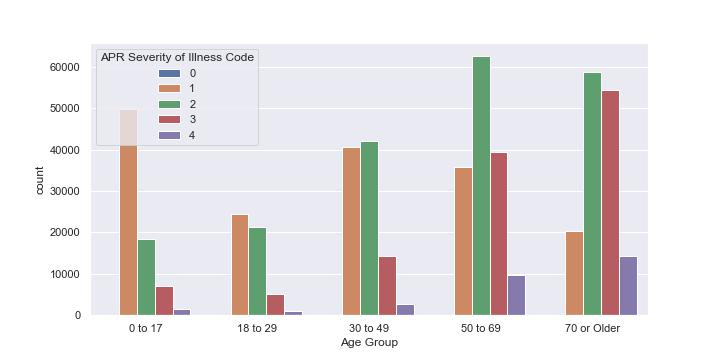
\includegraphics[height=13cm]{Figures/code-age_reduced.jpg} \\
\captionof{figure}{APR Severity of Illness Code associated with Age}\label{fig:code-age}%
\end{jdffigure}
\subsection{Difference between Original and Reduced Data}
When using 50\% of the data to create a reduced dataset, the number of data is only half of the original one. The frequency is in half in rough. Since the sampling the random, it is not exactly half. The histogram will show fewer data points and looks a little different compared to the histogram of the original dataset.
\subsection{Random Sampling influence}
Random sampling is a method where data points are selected randomly and uniformly from the original dataset, without considering any specific characteristic or attribute of the data points.
In this particular example, the data set is small and random sampling cut the origianla dataset in half. I believe the members from the age group are underrepresented in the original dataset, they may not be included in the reduced dataset and their frequency may be lower. In this case, the members from that age group may be harmed by the random sampling method.
\end{document}
